\subsection{Цель выполнения лабораторной работы}\label{blockN.VariantM}
\textbf{Цель выполнения лабораторной работы }-- \GoalOfResearch

%-------------------------------------------------
\subsection{Задание}
Для цепи Маркова, заданной стохастической матрицей переходов:
\begin{enumerate}
    \item нарисовать граф цепи;
    \item проверить выполнение критерия эргодичности;
    \item рассчитать предельные вероятности;
    \item записать предельную матрицу переходов;
    \item провести имитационное моделирование системы, соответствующей рассматриваемой цепи, для этого:
    \begin{itemize}
        \item случайно выбрать начальное состояние;
        \item случайно разыграть переход в новое состояние, учитывая распределение вероятностей перехода;
        \item совершить 100 переходов;
        \item повторить эксперимент 20 раз;
        \item подсчитать число вхождений в каждое из состояний системы;
        \item  построить <<графики>> переключений состояний цепи (для наглядности соединяем дискретные точки);
        \item составить таблицу для сравнения относительных частот наблюдений вхождения в каждое из состояний системы, указав исправленные оценки среднеквадратичных отклонений указанных относительных частот
    \end{itemize}
\end{enumerate}
%-------------------------------------------------
\newpage
\subsection{Решение}
Дана стохастическая матрица переходов $\mathbf{P}$:
$$\mathbf{P}=\begin{pmatrix}
0.26 & 0.15 & 0.2 & 0.21 & 0.18 \\
0.28 & 0.17 & 0.18 & 0.19 & 0.18 \\
0.21 & 0.13 & 0.17 & 0.32 & 0.17 \\
0.29 & 0.2 & 0.13 & 0.17 & 0.21 \\
0.18 & 0.18 & 0.2 & 0.24 & 0.2
\end{pmatrix}$$

На рисунке \ref{graph} представлен граф переходов, соответствующий матрице $\mathbf{P}$.
\begin{figure}[!h]
\centerline{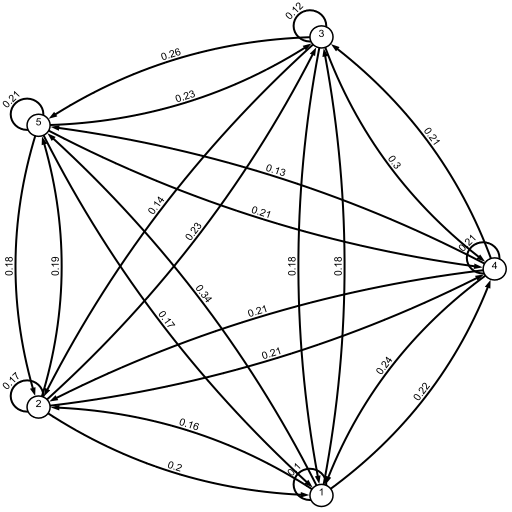
\includegraphics[width = 0.7\columnwidth]{Images/graph.png}}
\caption{Граф переходов}
\label{graph}
\end{figure}

\subsubsection{Определение вектора предельных вероятностей, проверка выполнения условия эргодичности}


$$(\mathbf{P}^T-\mathbf{E})\times\overline{p}=\overline{0},$$
где $\overline{p}$--вектор предельных вероятностей

Однако, поскольку система является линейно зависимой в качестве последнего уравнения внесем условие $\sum\limits_{i=1}^5p_i=1$.

Была реализована функция, вычисляющая вектор предельных вероятностей  $\overline{p}$, формирующая предельную матрицу переходов, а также проверяющая критерий эргодичности.

\begin{lstlisting}[language=python, label=prog,caption={\textit{расчет вектора предельных вероятностей}}]
def marginal_probabilities(P):
    A = P.T - np.eye(len(states), dtype=float)
    A[-1] = np.full(len(states), 1)
    b = np.zeros(len(states))
    b[-1] = 1.
    p = np.linalg.solve(A, b)
    return p, [list(p) for _ in range(len(states))], list(p).count(0)!=len(p)
\end{lstlisting}

~\\

Таким образом, вектор вектор предельных вероятностей:
$$\overline{p}=(0.24613\quad 0.16662\quad 0.17580\quad 0.22276\quad 0.18870)^T$$

Предельная матрица переходов:

$$\mathbf{P(n)}=\begin{pmatrix}
0.24613 & 0.16662 & 0.17580 & 0.22276 & 0.18870\\
0.24613 & 0.16662 & 0.17580 & 0.22276 & 0.18870\\
0.24613 & 0.16662 & 0.17580 & 0.22276 & 0.18870\\
0.24613 & 0.16662 & 0.17580 & 0.22276 & 0.18870\\
0.24613 & 0.16662 & 0.17580 & 0.22276 & 0.18870\\
\end{pmatrix} $$

~\\

\subsubsection{Имитационное моделирование}

Была разработана функция, реализующая переходы, заданное число раз, возвращающая траекторию и словарь с количеством посещений для каждого состояния (ключи--состояния).

\begin{lstlisting}[language=python, label=prog,caption={\textit{реализация марковского процесса}}]
def mark_iter(n, m, states):
    current_s = randrange(1,6)
    states_tr = [current_s]
    for _ in range(n-1):
        per_ver = m[current_s-1]
        next_s = np.random.choice(states, p=per_ver)
        current_s=next_s
        states_tr.append(current_s)
    return dict(sorted(dict(Counter(states_tr)).items())), states_tr
\end{lstlisting}

На рисунке \ref{iter} представлены «графики» переключений состояний цепи по результатам 20 экспериментов из 100 переходов.

\begin{figure}[!h]
\centerline{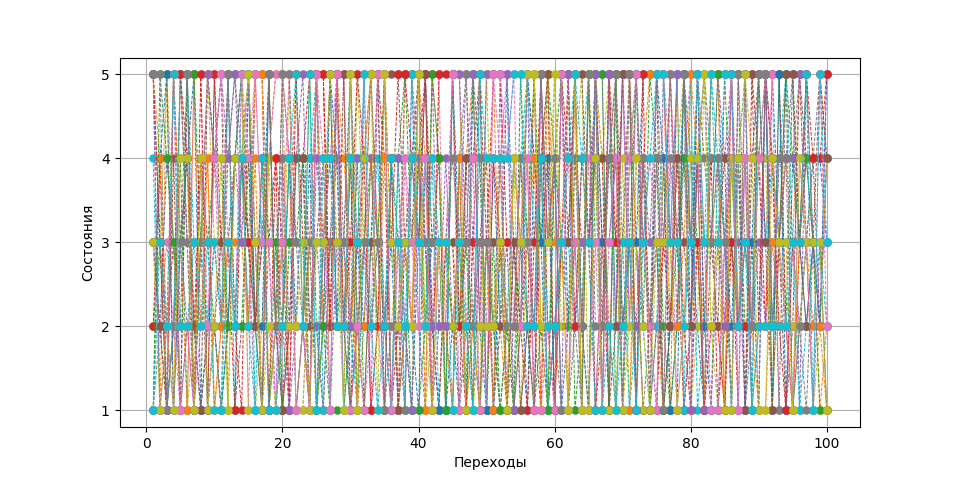
\includegraphics[width = \columnwidth]{Images/iter.png}}
\caption{Переключения состояния цепи}
\label{iter}
\end{figure}

В таблице \ref{table:Table_for_cheking_chislo_vlhozdeniy} представлено сранение относительных частот вхождения в каждое из состояний системы,
а также исправленные оценки среднеквадратичных отклонений указанных относительных частот, которое рассчитывается по формуле \ref{eq:1}.

\[
S = \sqrt{D \frac{n}{n-1}}
\tag{1} \label{eq:1}
\]

\begin{center}
\begin{table}[H]
\centering
\begin{tabular}{| c | c | c | c | c | c |}
\hline
№ & Сосотояние $S_1$ & Сосотояние $S_2$ & Сосотояние $S_3$ & Сосотояние $S_4$ & Сосотояние $S_5$ \\ \hline
  1 & 0.2 & 0.17 & 0.14 & 0.3 & 0.19 \\
 \hline 2 & 0.27 & 0.13 & 0.19 & 0.22 & 0.19 \\
 \hline 3 & 0.25 & 0.25 & 0.2 & 0.16 & 0.14 \\
 \hline 4 & 0.27 & 0.16 & 0.15 & 0.23 & 0.19 \\
 \hline 5 & 0.22 & 0.17 & 0.22 & 0.25 & 0.14 \\
 \hline 6 & 0.22 & 0.16 & 0.18 & 0.19 & 0.25 \\
 \hline 7 & 0.27 & 0.16 & 0.21 & 0.24 & 0.12 \\
 \hline 8 & 0.23 & 0.11 & 0.2 & 0.16 & 0.3 \\
 \hline 9 & 0.18 & 0.17 & 0.21 & 0.25 & 0.19 \\
 \hline 10 & 0.25 & 0.21 & 0.18 & 0.2 & 0.16 \\
 \hline 11 & 0.29 & 0.14 & 0.17 & 0.25 & 0.15 \\
 \hline 12 & 0.3 & 0.19 & 0.14 & 0.2 & 0.17 \\
 \hline 13 & 0.24 & 0.18 & 0.13 & 0.21 & 0.24 \\
 \hline 14 & 0.25 & 0.19 & 0.15 & 0.24 & 0.17 \\
 \hline 15 & 0.26 & 0.11 & 0.16 & 0.26 & 0.21 \\
 \hline 16 & 0.33 & 0.16 & 0.15 & 0.16 & 0.2 \\
 \hline 17 & 0.19 & 0.19 & 0.2 & 0.22 & 0.2 \\
 \hline 18 & 0.2 & 0.16 & 0.2 & 0.2 & 0.24 \\
 \hline 19 & 0.23 & 0.16 & 0.15 & 0.29 & 0.17 \\
 \hline 20 & 0.27 & 0.21 & 0.16 & 0.21 & 0.15 \\
 \hline \hline
S & 0.038 & 0.033 & 0.028 & 0.039 & 0.044 \\ \hline
\end{tabular}
\caption{Таблица для сравнения относительных частот наблюдений вхождения в каждое из состояний системы}
\label{table:Table_for_cheking_chislo_vlhozdeniy}
\end{table}
\end{center}


%-------------------------------------------------
\subsection{Вывод}
В ходе выполнения домашнего задания №1 была проанализирована работа марков- ского процесса, заданного стохастической матрицей переходов.

% --------------------------------------
% Атрибуты задачи
\labattributes{}{}{}{}{студент группы \EduGroup, \Author}{\Year, \Semestr}
%--------------
